 

This system relies on an external blockchain to initialize certain components. The system itself can be broken down into three main concepts which combined yield in its prevention of attacks. The goals that are ensured are described as:
\begin{itemize}
     \item \textbf{Security} - The ~safety~ and ~liveness~ properties of the TEE programs will be guaranteed.
     \item \textbf{Performance} - Achieving the security goals will not significantly impact performance. In detail, the aim is low latency for state updates and read operations, high throughput for processing enclave program requests, and unlimited state updates, provided by the blockchain.
\end{itemize} 
To start this section it is essential to mention that Narrator-Pro considers a distributed system if it at least holds \textit{n} = 2\textit{f} + 1 SGX-enabled instances in a cloud. Where \textit{f} is the number of faulty SEs, so the system can still properly work. The system can run a number (limited by specifications of the system) of enclaves which are divided into two groups of Application Enclaves (AEs) and State Enclaves (SEs). AEs have applications running, handle client requests, and return outputs corresponding to their inputs. SEs on the other hand contain the Narrator-Pro software and are responsible for providing state continuity to AEs. This is accomplished by a secure connection from the AE to a locally running SE, where the AE can use SEs Narrator-Pro libraries to seal data. This data is then used to retrieve the latest sealed state, in case of unexpected shutdowns. This principle is explained in more detail in §4.2. Figure ~\ref{fig:1} provides an overview of the mentioned components.

\begin{figure}[h]
    \centering
    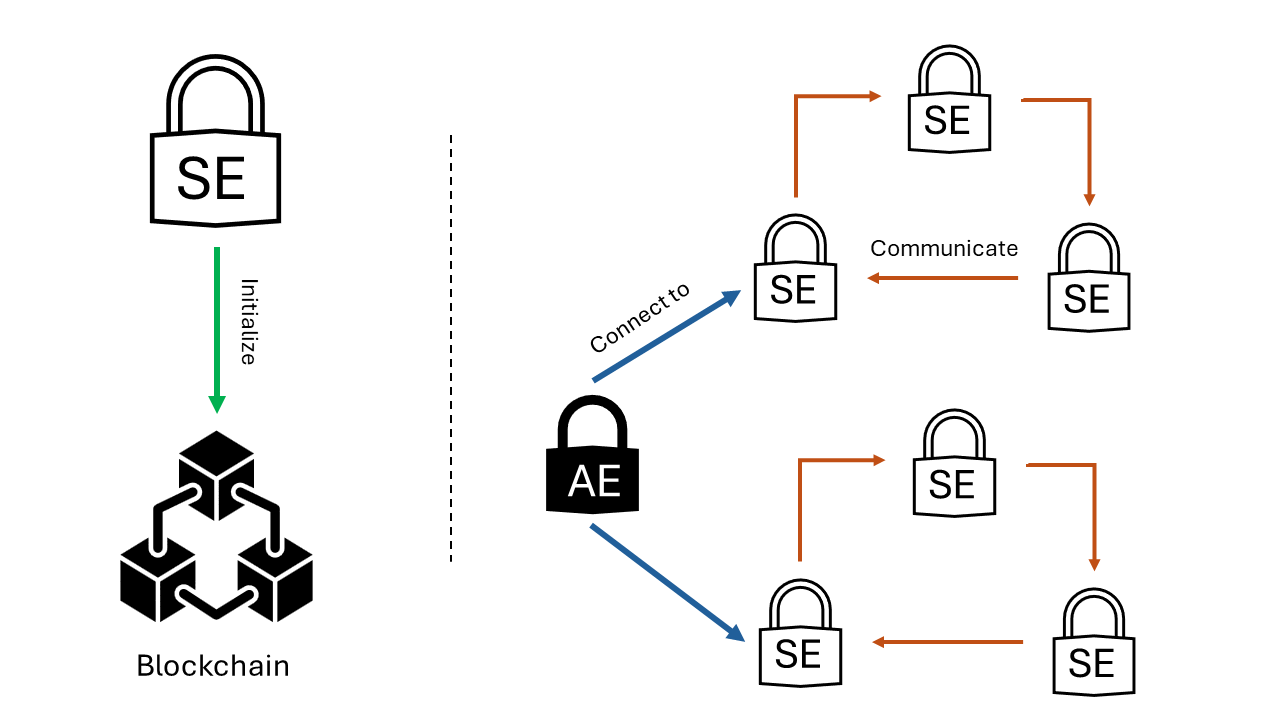
\includegraphics[width=\linewidth]{Figures/Figure1.png}
    \caption{The main components. The SE first has to initialize through the blockchain. Afterward, the groups will be established, where the AEs can link to}
    \label{fig:1}
\end{figure}


The authors also state a few premises which Narrator-Pro does. 
\begin{itemize}
    \item \textbf{Denial of Service Attacks} - It is not the goal to prevent systems from these kinds of attacks. Since TEEs themselves do not have prevention measures included.  
    \item \textbf{Hardware} - The implementation of Narrator-Pro should neither require any hardware changes nor will there be a need for specific hardware if the cloud TEE is already implemented.  
    \item \textbf{No Trusted Central Party} - Narrator-Pro does not rely on Trusted central parties, like trusted servers. However, since an external blockchain is used to initialize the system, the authors can not state that their system does not rely on Trusted Third Parties.
\end{itemize} 

The main concepts that constitute the reliance of Narrator-Pro are (1) system initialization §4.1, (2) state update and read protocols for AEs §4.2, and (3) restart protocols regarding AEs and SEs §4.3.

\subsection{System Initialization}

Before the system can start processing requests, it is essential to initialize the SEs. Adversaries will not be able to launch SEs with the same binary in the same group to get stale states. This is accomplished by the usage of a blockchain \textit{B}. 

The blockchain \textit{B} serves to store key-value tuples containing <\textit{key}, \textit{value}>. The \textit{value} is a random string linked to the \textit{key}, which will be returned by the blockchain in future read-calls. The, before mentioned, initialization process of SEs is carried out while the first write-call from a SE to \textit{B} is established. \textit{B} will verify that no other SE has registered on the blockchain with the provided \textit{key}. If this is the case the write-call will be executed and the client will receive an authenticator \textit{a}, with which he can verify the operation. This summarises the initialization responsibilities of \textit{B}.

The SE has to go through additional steps to finish its initialization. Therefore it is important to mention that SEs connect in groups to carry out requests delivered by AEs. Every group has an SE leader who is responsible for storing certain information about the group. If an SE wants to initialize, it first lets the leader establish a secure connection to itself. This connection channel spreads through the whole group so the participants can talk to each other. After the channel is in place, the initializing SE creates a key pair (which will be used in future connection establishments with this SE) and sends it to the leader, where it will be collected and stored in a list that is accessible for every SE in the group. Afterward, the before mentioned blockchain interaction takes place where the SE performs a read-call to \textit{B} and either receives the \textit{value} containing \textit{Null} (stating that no other SE has already linked to it with this \textit{key}) and the initialization succeeds or the SE terminates its initialization process. Subsequently, the first write-call will be executed where the SE stores its <\textit{key}, \textit{value}> tuple, and only then it can proceed to process the AE request.

\subsection{State Update and Read}

To prevent eavesdropping from adversaries, messages between AEs and SEs are transmitted over encrypted channels, using secret session keys. A nonce (Number used once) is sent as well to prevent replays. An AE will use an aforementioned group of SEs to confirm its current state \(S_i\), before proceeding with input \(I_i\) to update to \(S_{i+1}\). The following paragraphs will explain this procedure further (\(SD_{i}\) refers to the state digest, which is a summary of the latest states):

\begin{enumerate}
    \item \textbf{Input} - After receiving \(I_i\) from a user, the AE saves a state snapshot <\(S_i\), \(I_i\), \(SD_{i-1}\)> on the disk, in case the process crashes midway, so the current input/state can be retrieved. The AEs next step is to call the function (\textbf{writeState(\(SD_i\))} -> ACK) and wait for the returning ACK from the SE, to proceed with the state update.
    \item \textbf{writeState()} - With calling the \textbf{writeState()} function, the SE saves a snapshot of its states, containing <\(S_j\), \(I_j\), \(SD_{j-1}\)> with \(I_j\) = \(SD_{i}\). Upon a successful save, the SE starts communicating with its group by sending a PREPARE message <Prepare, \(SD_{j}\), (\textit{j}, \textit{seq})> to all SEs.\\
    The tuple <(\textit{j}, \textit{seq})> will be used in §4.3 for a rebooting SE to indicate if an enclave is active or was displaced by its clone.
    \item \textbf{PREPARE message} - Receiving a PREPARE message triggers the SE to update the sending SEs state digest in their memory. Consequently, an ECHO message is sent, containing \(SD_{j}\), signaling a successful update to the sending SE. Upon receiving \textit{f} + 1 ECHO messages, the initial SE adds the new state \(S_{i+1}\) to \(SD_{j+1}\) and sends an ACK to the AE. It then will advance its state to \(S_{i+1}\) and send the corresponding output to the user.
\end{enumerate}

A similar approach is used when an AE wants to verify the freshness of its current state. It calls the \textbf{readState()} function of its connected SE. The target SE, however, can not just return its current state digest (containing the latest states, with the freshest on top)
since due to a forking attack there could be more than one instance of this SE, holding stale state digests. So the creators of Narrator-Pro developed a sequence this SE has to run through, to verify its freshness:
\begin{enumerate}
    \item After calling \textbf{readState()} the target SE sends a request to all SEs in the group to obtain their saved state digests.
    \item Each SE then sends back the saved state digest, corresponding to the target SE, since every SE holds a list of all SE state digests, in the group.
    \item The target SE has to receive at least \textit{f} + 1 replies, where the state digest is the same as its, to be able to return it to the AE. 
\end{enumerate}


\subsection{Restart Protocol}
The last vulnerability that was discovered by the creators of Narrator-Pro is while an SE reboots and reconnects to its group, an adversary can leverage the group to perform a certain sequence, to enable forking and rollback attacks. This fact is best explained with an example, Figure  ~\ref{fig:2}. Consider three SEs \(S_{1}\), \(S_{2}\) and \(S_{3}\). With cloning \(S_{1}\) -> \(S'_{1}\) and \(S_{2}\) -> \(S'_{2}\) the initial enclaves will be displaced in the group by its copies, leaving \(S_{1}\) and \(S_{2}\) to be inactive. \(S_{3}\) will now communicate with the clones. However, the enclaves \(S_{1}\) and \(S_{2}\) do not know that they are inactive since the initial algorithm does not involve the necessity for the enclaves to know that they were displaced. This enables a copy of \(S_{3}\) -> \(S'_{3}\) to link to \(S_{1}\) and \(S_{2}\). This now leaves two groups, \textit{G1} and \textit{G2} of SEs. An adversary can now (1) increment the state with \textit{G1} and perform some actions leaving \textit{G2} with the old state and thereby rolling back the application. Or (2) feed two different inputs to \(S_{3}\) and \(S'_{3}\) and receive different outputs with 2 groups that have, respectfully the same binary, enabling a forking attack.\\
In order to prevent a system from performing this kind of sequence, the creators of Narrator-Pro included a requirement where an SE has to be confirmed by its group that at least \textit{f} SEs are not inactive, when reconnecting. This is accomplished by the tuple <(\textit{j}, \textit{seq})>, which is sent along with the \textbf{PREPARE messages}, where the index \textit{j} refers to the freshness of its state digest and \textit{seq} is used to distinguish different state digests with the same index.\\


\begin{figure}[h]
    \centering
    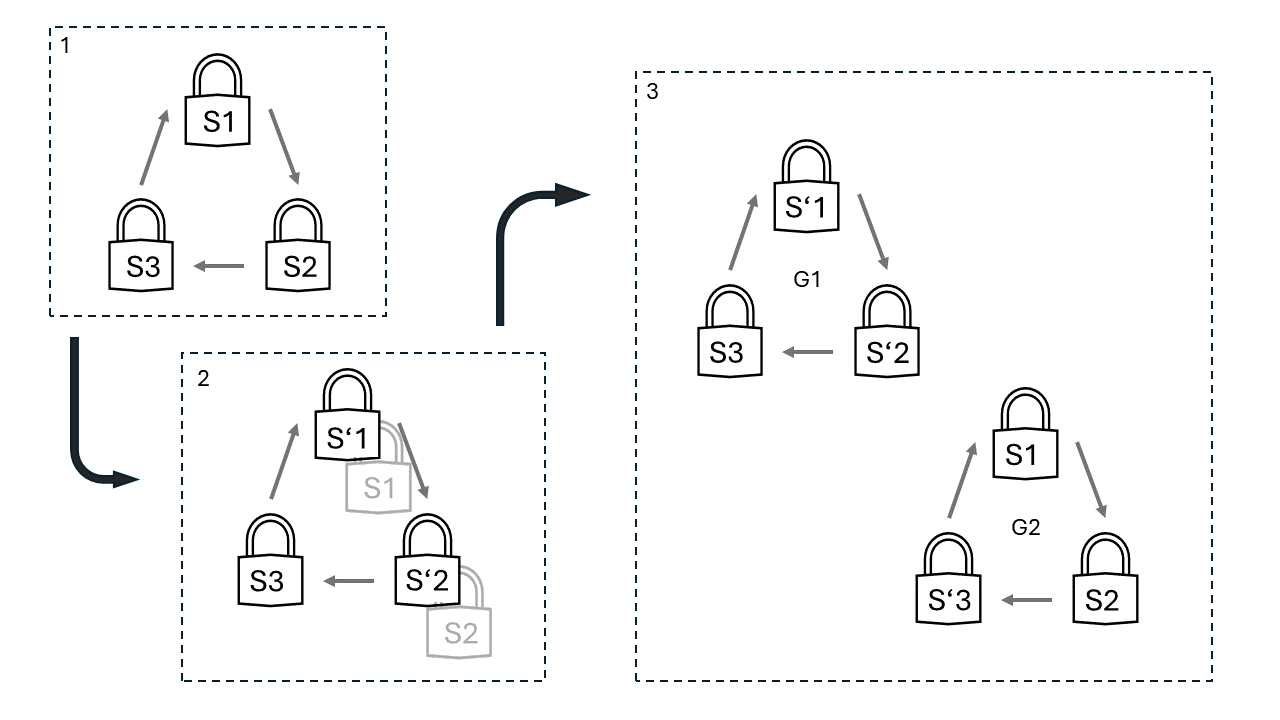
\includegraphics[width=\linewidth]{Figures/Figure2.png}
    \caption{The process of how to create forking groups}
    \label{fig:2}
\end{figure}